\documentclass{gajewski}

\bibliographystyle{IEEEtran}

%%%%%%%%%%%%%%%%%
% Document variables
%%%%%%%%%%%%%%%%%
\docDate{ \today }
\docID{Present cipher (32 bit input)}
\docRevision{0.2}
\docStatus{Draft}
\docTitle{\mbox{Present Cipher (32 bit input)}} 
\authorName{\mbox{Krzysztof Gajewski} \\ and opencores.org}
\authorURL{www.opencores.org}
\authorAddress{\mbox{}}
\authorEmail{gajos@opencores.org}

\revisionList{ 
0.1 & all & 2014/09/05 & First draft & K. Gajewski \\
0.2 & all & 2014/09/16 & Some small corrections with the text, typos, etc. & K. Gajewski \\
}

\begin{document}

\maketitle

\newpage

\revisionTable

\newpage

\tableofcontents
\newpage

\section{Introduction}

Present is \textgravedbl ultra-lightweight\textacutedbl \space block cipher developed by A. Bogdanov et al. and proposed in 2007 \cite{PRESENT}. It uses 64 bit data block and 80 bit or 128 bit key.
This cipher consists of 32 rounds, during which: 
\begin{itemize}
    \item round key is added to plaintext
    \item plaintext goes through sBoxes (substitution boxes)
    \item plaintext after sBoxes goes through pLayer (permutation layer)
    \item round key is updated
\end{itemize}
After that, ciphertext feeds out the output. Briefly algorithm was shown in Fig. \ref{pAlgorithm}.
\begin{figure}[!ht]%
    \begin{center}
    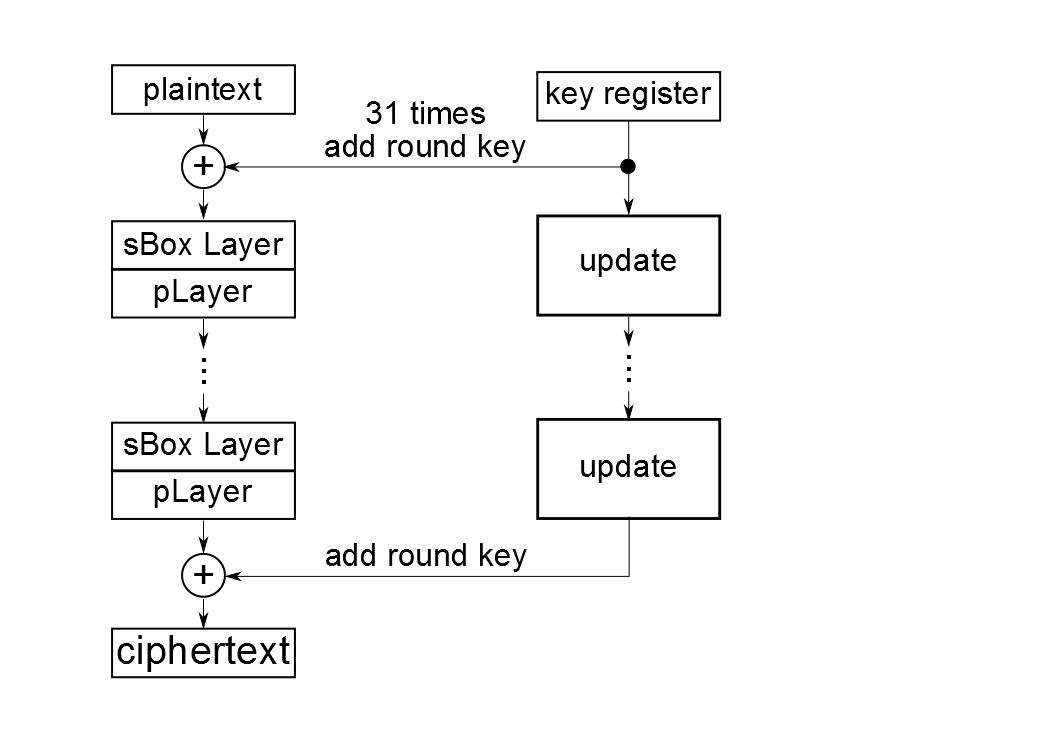
\includegraphics[width=0.66\textwidth]{img/presentAlgorithm.png}
    \caption{%
        Briefly block scheme of the PRESENT block cipher
     }%
    \label{pAlgorithm}
    \end{center}
 \end{figure}
In this project Present block cipher works with 80 bit key. Target was Xilinx\textsuperscript{\textregistered} Spartan 3E XC3S500E \cite{Spartan} on Spartan 3E  Starter Board \cite{Digilent} made by Digilent\textsuperscript{\textregistered}. In comparison with "plain" Present cipher project, this core was modified to take 32 bit word at input (plus control word). Output is also 32 bit.

\textbf{NOTE:}

This is rather "historical" project and is not recommended for future use.

\newpage 

\section{Interface}

Top level component of the Present component with 32 bit input was shown in Fig. \ref{penc}. All inputs and outputs are synchronous except \texttt{reset} signal and sampled at rising edge of the clock. Type for all signals is \texttt{STD\_LOGIC} or \texttt{STD\_LOGIC\_VECTOR}.
\begin{figure}[!ht]%
    \begin{center}
    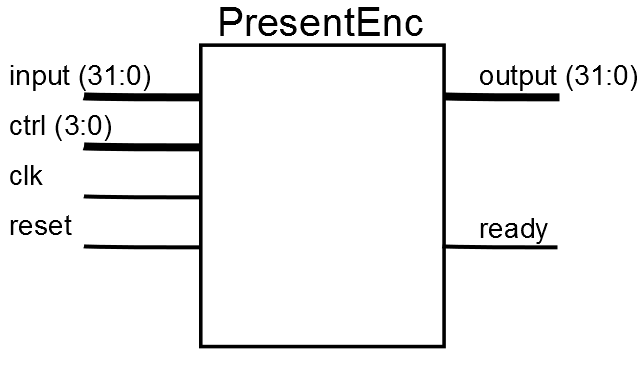
\includegraphics[width=0.5\textwidth]{img/PresentEnc.png}
    \caption{%
        Top level of the Present component with 32 bit input
     }%
    \label{penc}
    \end{center}
 \end{figure}

\begin{tabularx}{\textwidth}{|p{30mm}|p{11mm}|p{11mm}|X|}
  \hline \bf{Signal name} & \bf{Width} & \bf{In/Out} & \bf{Description}\\ 
  \hline \texttt{input}	& 32  &  in  & input data - both key and plaintext. \\ 
  \hline \texttt{ctrl}	& 4  &  in  & control bus for sending commands to the core. \\ 
  \hline \texttt{clk}	& 1  &  in  &  clock signal for the component\\ 
  \hline \texttt{reset} & 1   &  in  & \emph{asynchronous} reset signal.	\\ 
  \hline \texttt{output} & 32   &  out  & output data - ciphertext. \\ 
  \hline \texttt{ready} & 1   &  out  & signal informing about end of encoding process. \newline  "0" - wait until end of data encoding. \newline  "1" - end of the encoding process, output data available. \\ 
  \hline
\end{tabularx}
\captionof{table}{Input/Output signals of the Present component with 32 bit input}

\newpage

\section{State machine workflow}

Overall internal structure of the Present component with 32 bit input is similar to the structure shown in \cite{PRESENT}. To conform 64 bit plaintext, 80 bit key and 32 bit output data, multiplexer-like blocks was added to fit data. Additionally, control logic was added in the state machine. It was shown in Fig. \ref{presentSM}.

\begin{figure}[!ht]%
    \begin{center}
    \includegraphics[width=0.5\textwidth]{img/SM.jpg}
    \caption{%
        State machine of the Present component
     }%
    \label{presentSM}
    \end{center}
 \end{figure}

State machine consist of nine states \texttt{NOP}, \texttt{RDK1}, \texttt{RDK2}, \texttt{RDK3}, \texttt{RDT1}, \texttt{RDT2}, \texttt{COD}, \texttt{CTO1}, \texttt{CTO2}. \texttt{NOP} is the default state after resetting the core. This state is active as long as control bus (\texttt{ctrl}) don't have \texttt{crdk1} command at the input.

\texttt{RDKx} states are responsible for reading the key from the input. They are changing when suitable command appears at the \texttt{ctrl} input (\ref{presentSM}). When another commands appear, the state is changing to the \texttt{NOP} state. When command are left constant, given state is not changing.

\texttt{RDTx} states are responsible for reading the plaintext from the input. They are changing when suitable command appears at the \texttt{ctrl} input (\ref{presentSM}). When another commands appear, the state is changing to \texttt{NOP} state. When command are left constant, given state is not changing.

During the \texttt{COD} state encoding process start. If encoding process ends (after 32 clock cycles, \texttt{info = "00"} signal from the counter), state machine automaticly goes to the \texttt{CTO1} state. When commands another than \texttt{ccod} appear, the state is changing to the \texttt{NOP} state. When command are left constant encoding process is working.

\texttt{CTOx} states are responsible for sending the ciphertext to the output. They are changing when suitable command appears at the \texttt{ctrl} input (\ref{presentSM}). When another commands appear, the state is changing to the \texttt{NOP} state. When command are left constant, given state is not changing.

\newpage

\section{FPGA implementations}

The  component  has  only  been  verified on a Xilinx\textsuperscript{\textregistered} Spartan 3E XC3S500E FPGA in FG320 package and synthesized  with  Xilinx  ISE  14.2.  Appropriate setup files was prepared with the use of ISE Project Navigator, but Makefile scripts was also written. Suitable files was stored in \texttt{./32BitIO/syn/XC3ES500/} directory. Implementation in FPGA device \textbf{was not done} in this project (due to rather historical issues and nonconventional build of these core). Makefile was tested in Windows 8 with the use of Cygwin for 64-bit Windows.

Synthesis results was given in Fig. \ref{SynResults}

\begin{tabularx}{\textwidth}{|p{45mm}|p{30mm}|p{30mm}|X|}
  \hline \multicolumn{4}{|c|}{Xilinx \textregistered Spartan 3E XC3S500E FPGA in FG320 package} \\
  \hline \bf{Parameter} & \bf{Used} & \bf{Available} & \bf{Utilization}\\ 
  \hline Number of Slices & 313 & 4656 & 6\% \\
  \hline Number of Slice Flip Flops & 262 & 9312 & 2\% \\
  \hline Number of 4 input LUTs & 460 & 9312 & 4\% \\
  \hline Number of bonded IOBs & 71 & 232 & 30\% \\
  \hline Number of GCLKs & 1 & 24 & 4\%\\
  \hline Minimum period & 4.250 ns & - & - \\
  \hline Maximum Frequency & 235 MHz & - & - \\
  \hline
\end{tabularx}
\label{SynResults}
\captionof{table}{Synthesis results for Spartan 3E XC3S500E}

Possible change in used FPGA device may be possible in steps given below\footnotemark[1]:
\begin{enumerate}
    \item Copy \texttt{./32BitIO/syn/XC3ES500/} directory to another one like \texttt{./32BitIO/syn/YOUR\_FPGA\_SYMBOL/}
    \item Go to \texttt{./32BitIO/syn/YOUR\_FPGA\_SYMBOL/}  directory.
    \item In \texttt{PresentEnc.xst} file modify the line \texttt{-p xc3s500e-5-fg320} to \texttt{-p YOUR\_FPGA\_CODE}
    \item In \texttt{Makefile} file modify the line \texttt{PLATFORM=xc3s500e-fg320-5} to \texttt{PLATFORM=YOUR\_FPGA\_CODE}
\end{enumerate}

\footnotetext[1]{This solution was not tested and is based on my own observations.}

\newpage

\section{Simulation}

Self-checking test bench were provided to the components used for Present encoder. In case of whole Present with 32 bit input encoder this test bench was not self-checking. This is due to historical character of this project. They are stored in \texttt{./32BitIO/bench/vhdl} directory. Suitable configuration files and Makefile used for running test bench was stored in 
\texttt{./32BitIO/sim/rtl\_sim/bin} directory. Appropriate test vectors was taken from \cite{PRESENT}.

Makefile was prepared to make "manual run" of tests. If You want to perform it without gui, remove \texttt{-gui} option in Makefaile.

\newpage

\section{Troubleshooting}

During work with Windows 8 64-bit and and Xilinx\textsuperscript{\textregistered} ISE 64-bit some problems may occur:

\begin{enumerate}
    \item Xilinx may be unable to open projects in Project Navigator.
    \item When you run \texttt{make} in Cygwin and perform testbench it would be unable to open ISIM gui.
    \item When you run ISIM gui  (*.exe test bench file) it hangs out or anti virus protection opens.
\end{enumerate}

To solve problems listed above you have to perform steps listed below:
\begin{enumerate}
    \item You have to rename libraries \texttt{libPortabilityNOSH.dll} to \texttt{libPortability.dll} from \texttt{nt64} directories (\href{http://www.gadgetfactory.net/2013/09/having-problems-installing-xilinx-ise-on-windows-8-64bit-here-is-a-fix-video-included/}{http://www.gadgetfactory.net/2013/09/having-problems-installing-xilinx-ise-on-windows-8-64bit-here-is-a-fix-video-included/})
    \item Firstly, install Cygwin X11 (\href{http://stackoverflow.com/questions/9393462/cannot-launch-git-gui-using-cygwin-on-windows}{http://stackoverflow.com/questions/9393462/cannot-launch-git-gui-using-cygwin-on-windows})
    \item Temporary switch off anti virus protection.
\end{enumerate}

\newpage

\section{License and Liability}

Copyright \textcopyright  2013 Authors and OPENCORES.ORG

This source file may be used and distributed without
restriction provided that this copyright statement is not
removed from the file and that any derivative work contains
the original copyright notice and the associated disclaimer.

This source file is free software; you can redistribute it
and-or modify it under the terms of the GNU Lesser General
Public License as published by the Free Software Foundation;
either version 2.1 of the License, or (at your option) any
later version.

This source is distributed in the hope that it will be
useful, but WITHOUT ANY WARRANTY; without even the implied
warranty of MERCHANTABILITY or FITNESS FOR A PARTICULAR
PURPOSE. See the GNU Lesser General Public License for more
details.

You should have received a copy of the GNU Lesser General
Public License along with this source; if not, download it
from \href{http://www.opencores.org/lgpl.shtml}{http://www.opencores.org/lgpl.shtml}

Xilinx, Spartan3E is registered trademark of Xilinx Inc. 2100 Logic Drive, San Jose CA USA

\newpage

\bibliography{bibliography}

\end{document}
